\chapter{Implementacija i korisničko sučelje}


		\section{Korištene tehnologije i alati}

		Pri izradi dokumentacije korišten je \textbf{LaTeX}\footnote{\url{https://www.latex-project.org/}} - visokokvalitetan sustav za pisanje teksta koji uključuje značajke dizajnirane za izradu tehničke i znanstvene dokumentacije. Za izradu dokumenta korišteno je integrirano okruženje \textbf{TeXstudio}\footnote{\url{https://www.texstudio.org/}} namijenjeno izradi LaTeX dokumenata. \\ \\
			Dijagrami u sklopu dokumentacije izrađeni su s \textbf{Astah}\footnote{\url{https://astah.net/}} alatom za UML modeliranje. \\ \\
			Za izradu backend-a aplikacije korišten je objektno orijentirani programski jezik \textbf{Java(19)}\footnote{\url{https://www.java.com/en/}} te radni okvir \textbf{Spring Boot}\footnote{\url{https://spring.io/}} - aplikacijski okvir otvorenog koda koji pruža infrastrukturnu podršku za razvoj Java aplikacija. Backend smo testirali s platformom za testiranje API-ja \textbf{Postman}\footnote{\url{https://www.postman.com/}}. \\ \\
			 Za izradu frontend-a korišten je skriptni programski jezik \textbf{JavaScript}\footnote{\url{https://www.javascript.com/}} koji se izvršava u web pregledniku na strani korisnika te \textbf{ReactJS}\footnote{\url{https://reactjs.org/}} - frontend JavaScript biblioteka otvorenog koda za izgradnju korisničkih sučelja temeljenih na UI komponentama. Sav programski kod napisan je u integriranom razvojnom okruženju za razvoj računalnog servera \textbf{IntelliJ IDEA}\footnote{\url{https://www.jetbrains.com/idea/}}. \\ \\
			Za izradu baze podataka korišten je sustav za upravljanje bazama podataka \textbf{PostgreSQL}\footnote{\url{https://www.postgresql.org/}}. Pristup bazi izvršavan je putem SQL klijentskih aplikacija i alata za administraciju baze podataka \textbf{DBeaver}\footnote{\url{https://dbeaver.io/}} i \textbf{pgAdmin 4}\footnote{\url{https://www.pgadmin.org/}} \\ \\
			 Za upravljanje projektom te online pohranu programskog koda i dokumentacije korišten je \textbf{GitLab}\footnote{\url{https://about.gitlab.com/}} - repozitorij otvorenog koda i platforma za kolaborativni razvoj softvera. Članovi tima su za međusobnu komunikaciju koristili aplikacije \textbf{WhatsApp}\footnote{\url{https://www.whatsapp.com/}} i \textbf{Discord}\footnote{\url{https://discord.com/}}.

		\eject


		\section{Ispitivanje programskog rješenja}

		\subsection{Ispitivanje komponenti}
		\textit{Ispitivanje komponenti proveli smo pomoću Selenium WebDrivera (\url{https://www.selenium.dev/documentation/webdriver/}) unutar JUnit testova kao podršku za pisanje ispita unutar programskog jezika Java. }

		\bigskip

		\textit{Pomoću Selenuima izradili smo 6 ispitnih slučajeva. U prvome ispitnom slučaju prikazanom na provjerena je funkcionalnost gumba za prijavu na početnoj stranici, čija funkcionalnost je rezultirala ispravnim testom.}

		\begin{small}


		\noindent{
			\begin{lstlisting}[language=Java] \\
				@Test \\
				public void testNavBarLogin() { \\
					System.setProperty("webdriver.chrome.driver", "src/test/java/cadl/globerunner/chromedriver"); \\
					WebDriver driver = new ChromeDriver(); \\
					driver.manage().timeouts().implicitlyWait(10, TimeUnit.SECONDS); \\
					driver.get("https://globerunnergame.onrender.com"); \\
					\\
					driver.findElement(By.className("nav-item")).click(); \\
					\\
					String redirURL = driver.getCurrentUrl(); \\
					\\
					boolean comperRes = redirURL.contains("/login"); \\
					\\
					assertEquals(comperRes, true); \\
					\\
					driver.quit(); \\
				}\\
			\end{lstlisting}}

		\end{small}

		\bigskip

		\textit{Drugi ispitni slučaj provjerava funkcionalnost klika na logo igre, pri čemu je ona ispravno provedena, rezultirajući sa odlaskom na početnu stranicu.}

		\begin{small}

		\noindent{
			\begin{lstlisting}[language=Java] \\
				@Test \\
				public void testGumbLogo() { \\
					System.setProperty("webdriver.chrome.driver", "src/test/java/cadl/globerunner/chromedriver"); \\
					WebDriver driver = new ChromeDriver(); \\
					driver.manage().timeouts().implicitlyWait(10, TimeUnit.SECONDS); \\
					driver.get("https://globerunnergame.onrender.com"); \\
					\\
					driver.findElement(By.className("nav-item")).click(); \\
					\\
					driver.findElement(By.className("navbar-brand")).click(); \\
					\\
					String redirURL = driver.getCurrentUrl(); \\
					\\
					boolean comperRes = redirURL.contains("https://globerunnergame.onrender.com"); \\
					\\
					assertEquals(comperRes, true); \\
					\\
					driver.quit(); \\
				} \\
		\end{lstlisting}}

		\end{small}

		\bigskip

		\textit{Treći ispitni slučaj provjerava funkcionalnost gumba za registraciju igrača na početnoj stranici, čija funkcionalnost je rezultirala ispravnim testom i odlaskom na stranicu za unos podataka.}

		\begin{small}

		\noindent{
			\begin{lstlisting}[language=Java] \\
				@Test \\
				public void testNavBarRegister() { \\
					System.setProperty("webdriver.chrome.driver", "src/test/java/cadl/globerunner/chromedriver"); \\
					WebDriver driver = new ChromeDriver(); \\
					driver.manage().timeouts().implicitlyWait(10, TimeUnit.SECONDS); \\
					driver.get("https://globerunnergame.onrender.com"); \\
					\\
					driver.findElement(By.className("nav-link dropdown")).click(); \\
					driver.findElement(By.partialLinkText("/registerP")).click(); \\
					\\
					String redirURL = driver.getCurrentUrl(); \\
					\\
					boolean comperRes = redirURL.contains("/registerP"); \\
					\\
					assertEquals(comperRes, true); \\
					\\
					driver.quit(); \\
				} \\
		\end{lstlisting}}


		\end{small}

		\bigskip

		\textit{Četvrti ispitni slučaj provjerava funkcionalnost ispravne prijave koja je rezultirala ispravnim testom i odlaskom na stranicu profila korisnika.}

		\begin{small}

		\noindent{
			\begin{lstlisting}[language=Java] \\
				@Test  \\
				public void testGoodLoginCreds() {  \\
					System.setProperty("webdriver.chrome.driver", "src/test/java/cadl/globerunner/chromedriver");  \\
					WebDriver driver = new ChromeDriver();  \\
					driver.manage().timeouts().implicitlyWait(10, TimeUnit.SECONDS);  \\
					driver.get("https://globerunnergame.onrender.com/login");  \\
					 \\
					WebElement element = driver.findElement(By.name("username"));  \\
					element.sendKeys("GrilBers");  \\
					 \\
					element = driver.findElement(By.name("password")); \\
					element.sendKeys("Putnik123"); \\
					 \\
					driver.findElement(By.className("btn")).click(); \\
					 \\
					String redirURL = driver.getCurrentUrl(); \\
					 \\
					boolean comperRes = redirURL.contains("https://globerunnergame.onrender.com/prijave"); \\
					 \\
					assertEquals(comperRes, true); \\
					 \\
					driver.quit(); \\
				} \\
		\end{lstlisting}}


		\end{small}

		\bigskip


		\textit{Peti ispitni slučaj provjerava funkcionalnost neispravne prijave koja je rezultirala ispravnim testom i očekivanim ostajanjem na stranici prijave.}

		\begin{small}

		\noindent{
			\begin{lstlisting}[language=Java] \\
				@Test \\
				public void testBadLoginCreds() { \\
					System.setProperty("webdriver.chrome.driver", "src/test/java/cadl/globerunner/chromedriver"); \\
					WebDriver driver = new ChromeDriver(); \\
					driver.manage().timeouts().implicitlyWait(10, TimeUnit.SECONDS); \\
					driver.get("https://globerunnergame.onrender.com/login"); \\
					\\
					WebElement element = driver.findElement(By.name("username")); \\
					element.sendKeys("Pulin Vulin"); \\
					\\
					element = driver.findElement(By.name("password")); \\
					element.sendKeys("Poludi Ivice"); \\
					\\
					driver.findElement(By.className("btn")).click(); \\
					\\
					String redirURL = driver.getCurrentUrl(); \\
					\\
					boolean comperRes = redirURL.contains("/login"); \\
					\\
					assertEquals(comperRes, true); \\
					 \\
					driver.quit(); \\
				} \\
		\end{lstlisting}}

		\end{small}

		\bigskip

		\textit{Na kraju zadnji ispitni slučaj provjerava funkcionalnost prijave, te gumba za započinjanje borbe na stranici profila, pri čemu su obje funkcionalnosti pokazale se ispravnima i aplikacija je rezultirala ispravnim odlaskom na stranicu borbe.}

		\begin{small}

		\noindent{
			\begin{lstlisting}[language=Java] \\
				@Test \\
				public void testZapocniBorbu() { \\
					System.setProperty("webdriver.chrome.driver", "src/test/java/cadl/globerunner/chromedriver"); \\
					WebDriver driver = new ChromeDriver(); \\
					driver.manage().timeouts().implicitlyWait(10, TimeUnit.SECONDS); \\
					driver.get("https://globerunnergame.onrender.com"); \\
					\\
					driver.findElement(By.className("nav-item")).click(); \\
					\\
					WebElement element = driver.findElement(By.name("username")); \\
					element.sendKeys("Juma"); \\
					\\
					element = driver.findElement(By.name("password")); \\
					element.sendKeys("12345"); \\
					\\
					driver.findElement(By.className("btn")).click(); \\
					\\
					driver.findElement(By.id("button-borba")).click(); \\
					\\
					String redirURL = driver.getCurrentUrl(); \\
					\\
					boolean comperRes = redirURL.contains("/borba"); \\
					\\
					assertEquals(comperRes, true); \\
					\\
					driver.quit(); \\
				} \\
		\end{lstlisting}}


		\end{small}

		\bigskip

		\subsection{Ispitivanje sustava}

		\textit{Ispitivanje sustava proveli smo pomoću Selenium WebDrivera (\url{https://www.selenium.dev/documentation/webdriver/}) unutar JUnit testova kao podršku za pisanje ispita unutar programskog jezika Java. }

		\bigskip

		\textit{Pomoću Selenuima izradili smo 4 ispitna slučaja. U prvome ispitnom slučaju prikazanom na provjerena je funkcionalnost prijave, pregleda profila i odjave, pri čemu je prijava bila uspješna te je funkcionalnost pregleda i odjave ostvarena.}

		\begin{small}

		\noindent{
			\begin{lstlisting}[language=Java] \\
				@Test \\
				public void testPrijavaProfilOdjava() { \\
					System.setProperty("webdriver.chrome.driver", "src/test/java/cadl/globerunner/chromedriver"); \\
					WebDriver driver = new ChromeDriver(); \\
					driver.manage().timeouts().implicitlyWait(10, TimeUnit.SECONDS); \\
					driver.get("https://globerunnergame.onrender.com"); \\
					 \\
					driver.findElement(By.className("nav-item")).click(); \\
					 \\
					WebElement element = driver.findElement(By.name("username")); \\
					element.sendKeys("Juma"); \\
					 \\
					element = driver.findElement(By.name("password")); \\
					element.sendKeys("12345"); \\
					 \\
					driver.findElement(By.className("btn")).click(); \\
					 \\
					driver.findElement(By.partialLinkText("/logged")).click(); \\
					 \\
					driver.findElement(By.className("log-out")).click(); \\
					 \\
					String redirURL = driver.getCurrentUrl(); \\
					 \\
					boolean comperRes = redirURL.contains("/login"); \\
					 \\
					assertEquals(comperRes, true); \\
					 \\
					driver.quit(); \\
				} \\
		\end{lstlisting}}


		\end{small}

		\bigskip

		\textit{Drugi ispitni slučaj provjerava funkcionalnost prijave kartografa, prijave lokacije te funkcionalnost klika na logo igre, pri čemu su sve tri funkcionalnosti ispravne i provedene, rezultirajući sa odlaskom na početnu stranicu.}

		\begin{small}

		\noindent{
			\begin{lstlisting}[language=Java] \\
				@Test \\
				public void testPrijavaLokacijeLogo() { \\
					System.setProperty("webdriver.chrome.driver", "src/test/java/cadl/globerunner/chromedriver"); \\
					WebDriver driver = new ChromeDriver(); \\
					driver.manage().timeouts().implicitlyWait(10, TimeUnit.SECONDS); \\
					driver.get("https://globerunnergame.onrender.com"); \\
					\\
					driver.findElement(By.className("nav-item")).click(); \\
					\\
					WebElement element = driver.findElement(By.name("username")); \\
					element.sendKeys("GrilBers"); \\
					\\
					element = driver.findElement(By.name("password")); \\
					element.sendKeys("Putnik123"); \\
					\\
					driver.findElement(By.className("btn")).click(); \\
					\\
					driver.findElement(By.className("navbar-brand")).click(); \\
					\\
					String redirURL = driver.getCurrentUrl(); \\
					\\
					boolean comperRes = redirURL.contains("https://globerunnergame.onrender.com"); \\
					\\
					assertEquals(comperRes, true); \\
					\\
					driver.quit(); \\
				} \\
		\end{lstlisting}}


		\end{small}

		\bigskip



		\textit{Treći ispitni slučaj provjerava funkcionalnost gumba borbe, pri čemu je njegova funkcionalnost i ostvarena odlaskom na stranicu borbe.}

		\begin{small}

		\noindent{
			\begin{lstlisting}[language=Java] \\
				@Test \\
				public void testGumbBorbe() { \\
					System.setProperty("webdriver.chrome.driver", "src/test/java/cadl/globerunner/chromedriver"); \\
					WebDriver driver = new ChromeDriver(); \\
					driver.manage().timeouts().implicitlyWait(10, TimeUnit.SECONDS); \\
					driver.get("https://globerunnergame.onrender.com"); \\
					 \\
					driver.findElement(By.className("nav-item")).click(); \\
					 \\
					WebElement element = driver.findElement(By.name("username")); \\
					element.sendKeys("Juma"); \\
					 \\
					element = driver.findElement(By.name("password")); \\
					element.sendKeys("12345"); \\
					 \\
					driver.findElement(By.className("btn")).click(); \\
					 \\
					driver.findElement(By.className("btn btn-outline-light")).click(); \\
					 \\
					driver.findElement(By.className("navbar-brand")).click(); \\
					 \\
					String redirURL = driver.getCurrentUrl(); \\
					 \\
					boolean comperRes = redirURL.contains("https://globerunnergame.onrender.com/borba"); \\
					 \\
					assertEquals(comperRes, true); \\
					 \\
					driver.quit(); \\
				} \\
		\end{lstlisting}}


		\end{small}

		\bigskip

		\textit{Četvrti ispitni slučaj provjerava funkcionalnost prijave igrača, te funkcionalnost prikaza rang liste, pri čemu su obje funkcionalnosti ispravne i provedene, rezultirajući sa odlaskom na stranicu za prikaz ranga.}

		\begin{small}

		\noindent{
			\begin{lstlisting}[language=Java] \\
				@Test \\
				public void testRangList() { \\
					System.setProperty("webdriver.chrome.driver", "src/test/java/cadl/globerunner/chromedriver"); \\
					WebDriver driver = new ChromeDriver(); \\
					driver.manage().timeouts().implicitlyWait(10, TimeUnit.SECONDS); \\
					driver.get("https://globerunnergame.onrender.com"); \\
					 \\
					driver.findElement(By.className("nav-item")).click(); \\
					 \\
					WebElement element = driver.findElement(By.name("username")); \\
					element.sendKeys("Juma"); \\
					 \\
					element = driver.findElement(By.name("password")); \\
					element.sendKeys("12345"); \\
					 \\
					driver.findElement(By.className("btn")).click(); \\
					 \\
					driver.findElement(By.partialLinkText("/rankList")).click(); \\
					 \\
					String redirURL = driver.getCurrentUrl(); \\
					 \\
					boolean comperRes = redirURL.contains("/rankList"); \\
					 \\
					assertEquals(comperRes, true); \\
					 \\
					driver.quit(); \\
				} \\
		\end{lstlisting}}


		\end{small}

		\eject


		\section{Dijagram razmještaja}

			Specifikacijski dijagrami razmještaja prikazuju pregled implementacije artefakata bez upućivanja na specifične slučajeve artefakata. Na poslužiteljskom računalu se nalaze web poslužitelj. Klijenti koriste web preglednik kako bi pristupili web aplikaciji. Sustav je baziran na arhitekturi ”klijent – poslužitelj”, a komunikacija između računala korisnika i poslužitelja odvija se preko HTTP veze. Baza podataka se nalazi na vanjskom uređaju (serveru) te njoj pristupa back-end web aplikacije s poslužiteljskog računala.
			\begin{figure}[H]
				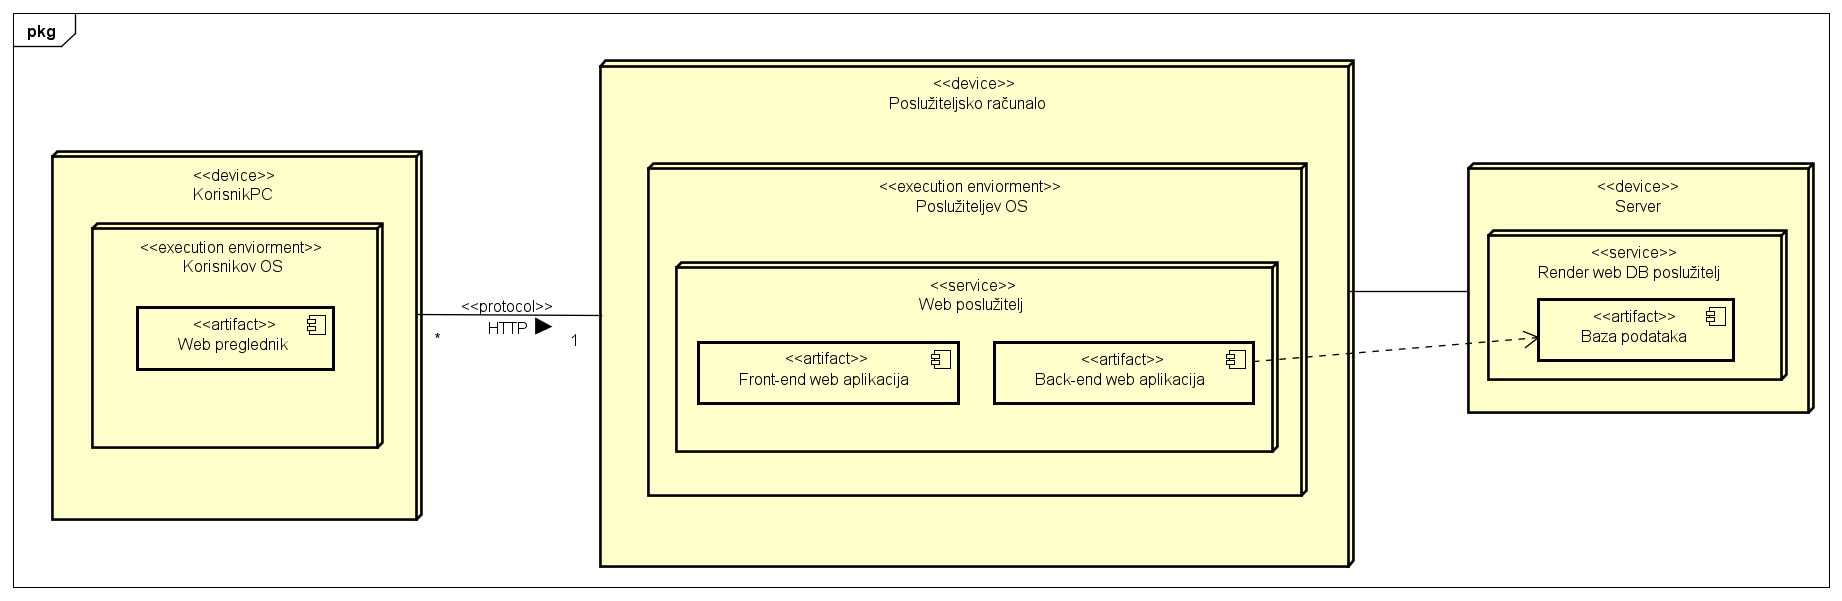
\includegraphics[width=\textwidth]{slike/Dijagram_razmjestaja.png}
				\centering
				\caption{Dijagram razmjestaja}
				\label{fig:promjene}
			\end{figure}
			\eject

		\section{Upute za puštanje u pogon}

			Aplikacija je dostupna na mreži na linku \url{https://globerunnergame.onrender.com/}. Za postavljanje aplikacije na mrežu koristili smo Render. Na main grani je dostupna konfiguracija potrebna za puštanje u pogon preko Render-a. U ovom dijelu ćemo opisati kako se aplikacija pokreće lokalno. Za pokretanje aplikacije lokalno, treba se prebaciti u dev granu.

			\subsection{Baza podataka}

			Baza podataka je postavljena na Render-u te se i kada lokalno pokrećemo aplikaciju, aplikacija spaja na tu bazu. Baza koristi PostgreSQL verziju 15. Sljedeći parametri su potrebni za spajanje na bazu:

			\begin{itemize}
				\item Hostname - dpg-cdn6t5la49944a9s62ug-a.frankfurt-postgres.render.com
				\item Port - 5432
				\item Database - globerunner\_bb6l
				\item Username - admin
				\item Password - 9C4cZ3gth11MaaVCKegvGJxVVjwOVgEq
			\end{itemize}

			\bigskip

			\subsection{Back-end aplikacija}

			Back-end web aplikacija je Java Spring Boot projekt. Za pokretanje servera potrebno je na računalu imati instalirano Java Development Kit 19 koji sadrži virtualni stroj koji može pokrenuti aplikaciju i prevoditelja koji može prevesti kod za taj virtualni stroj. Projektu u izgradnji i pokretanju pomaže alat Maven. U datoteci pom.xml zapisane su sve biblioteke koje smo trebali za projekt. Maven instalirava potrebne biblioteke. Za kraj se trebaju postaviti podatci za spajanje na bazu. U datoteci src/main/resources/application.properties postavljaju se parametri:

			\begin{itemize}
				\item spring.datasource.password=9C4cZ3gth11MaaVCKegvGJxVVjwOVgEq
				\item spring.datasource.username=admin
				\item spring.datasource.url=jdbc:postgresql://dpg-cdn6t5la49944a9s62ug-a.frankfurt-postgres.render.com:5432/globerunner\_bb6l
				\item spring.datasource.driverClassName=org.postgresql.Driver

				\item spring.jpa.show-sql=true
				\item spring.jpa.hibernate.ddl-auto=update
				\item spring.jpa.properties.hibernate.dialect=org.hibernate.dialect.PostgreSQLDialect
				\item spring.jpa.properties.hibernate.format\_sql=true
			\end{itemize}

			Za pokretanje aplikacije, potrebno je pokrenuti razred \\ src/main/java/cadl/globerunner/GloberunnerApplication.java.

			\bigskip

			Za puštanje aplikacije na Render potrebno je napraviti Docker file od kojeg se može složiti sustav kontejner koji će pokretati aplikaciju.

			\bigskip

			\subsection{Front-end aplikacija}

			Front-end web aplikacija je React projekt. Za pokretanje servera potrebno je na računalu imati instaliran Node.js i npm (Node Package Manager). Za početak je potrebno instalirati sve dodatne node module koje smo koristili u projektu tako da se u terminal pozicioniran u root folderu projekta upiše npm install --legacy-peer-deps. Kada su instalirani moduli, možemo pokrenuti server tako da upišemo u terminal npm run start.

			Svi HTTP zahtjevi za back-end šalju se na localhost:8080/.


			\eject
